\documentclass[10pt]{article}\usepackage[margin=.55in]{geometry}\usepackage[T1]{fontenc}\usepackage{graphicx}\setlength{\parindent}{0pt}\setlength{\parskip}{4pt}\sloppy\begin{document}{\large Saved signed-collector scheduler reconstruction}\par Software validation, 2 November 2026. Six saved streams pass deterministic scheduler reconstruction: 731 candidate transitions and 363 choices. Three deliberately altered streams pass the existing graph and group-label checks but are rejected by the scheduler check.\par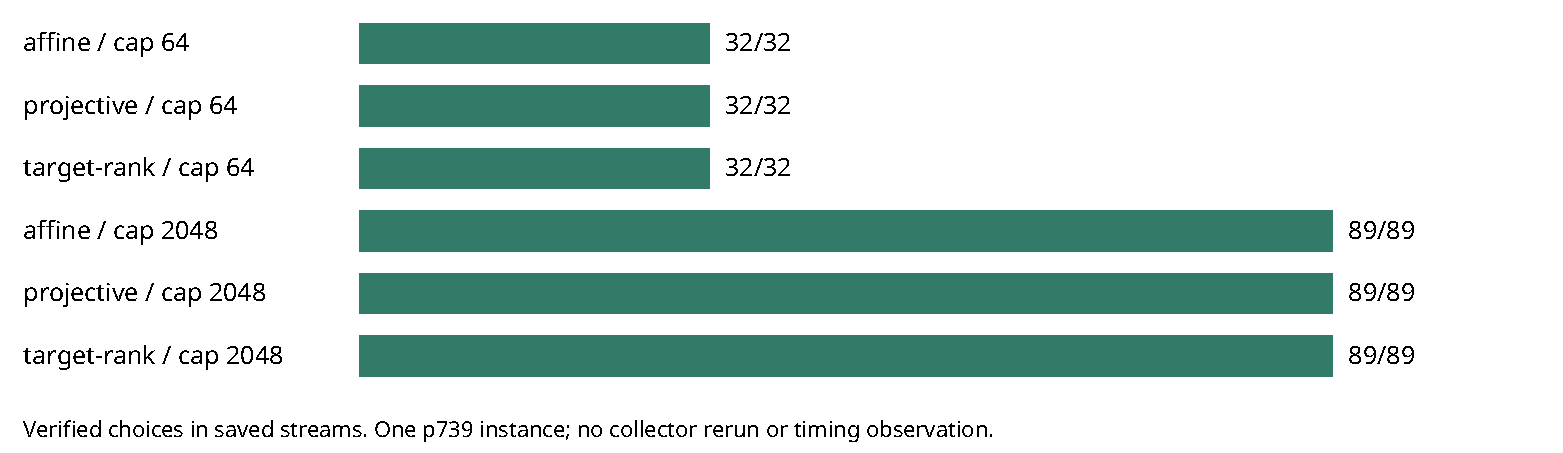
\includegraphics[width=.9\linewidth]{diagram.pdf}\par The verifier reconstructs sixteen jumps and the starting state from the header seed using a separately written SplitMix64 and bounded uniform draw routine. It checks each jump index, candidate divisor and scalar-label transition, and first-maximal candidate selection. Affine Cantor arithmetic checks both affine and projective-labelled streams. Connectivity priorities use direct component-member relabelling rather than the producer's union-find. Rank priorities use the preceding strict graph replay's checked native rank score.

The six inputs are the existing p=739, target 2G controls: affine, projective and target-rank variants at caps 64 and 2048. Candidate counts are 64, 64, 64, 180, 180 and 179. Choice counts are 32, 32, 32, 89, 89 and 89. Each short stream consumes 66 reconstructed random draws; each long stream consumes 124. Three recorded source scalars verify. These are saved software controls, not a new cohort or cost measurement.

The negative controls change the header seed (and supplied expected header), a valid distinct jump index, or the selected candidate. Each still passes graph and group-label validation; the scheduler rejects them respectively for a candidate-state, jump-index, or first-maximal-choice mismatch. Changing both copies of the seed is a test of internal consistency, not authenticated-header custody.

All two integration tests and exact source-binding checks pass. Formatting checks pass. Raw logs, source hashes and per-stream CSV and JSON retain the evidence. No collector, container or scientific worker was launched.

Both restart paths are implemented but none of these six native streams contains a restart. Their scheduler reconstruction therefore has no positive restart-path coverage yet. The separately published constructed exceptional controls establish graph and label coverage, not native scheduler provenance. Cantor arithmetic and native rank scoring are shared dependencies; independent source-fidelity review remains pending.
\end{document}